\documentclass[12pt,twoside]{article}

% Language setting
% Replace `english' with e.g. `spanish' to change the document language
\usepackage[english]{babel}

% Set page size and margins
% Replace `letterpaper' with `a4paper' for UK/EU standard size
\usepackage[letterpaper,top=2cm,bottom=2cm,left=3cm,right=3cm,marginparwidth=1.75cm]{geometry}

% Useful packages
\usepackage{mathptmx} %% For TImes New Roman Font
\usepackage{amsmath}
\usepackage{graphicx}
\usepackage[colorlinks=true, allcolors=blue]{hyperref}
%\usepackage{fancyhdr}

\title{Title: Development of a Low-Power Keyword Spotter (KWS) for "Bleeding-Edge" Applications}
\author{Design Contest, VLSID 2025, Bengaluru}

\begin{document}
\maketitle

\begin{abstract}

\end{abstract}

%%%--- HARDWARE PLATFORM
\section{Hardware Platform}

\subsubsection*{Microchip Technology’s RISC-V based PolarFire SoC Icicle Kit}

The \href{https://www.microchip.com/en-us/development-tool/mpfs-icicle-kit-es}{PolarFire SoC Icicle Kit} is a low-cost platform for evaluating the five-core Linux-capable RISC-V microprocessor subsystem, real-time execution, low-power capabilities, and peripherals of the PolarFire SoC FPGA. PolarFire SoC is ideal for power-efficient computing in applications such as audio, AI/ML, industrial automation, and IoT. The Icicle kit includes onboard memories (LPDDR4, SPI, eMMC flash) for Linux, a multi-rail power sensor, PCIe root port, Raspberry Pi, mikroBUS expansion ports, and various wired connectivity options for prototyping.


%%%--- EXPLANATION OF IDEA
\section{Explanation of the Idea}
% Include a block diagram, overview of implementation  (Minimum font size: 10pt, Times New Roman font. Maximum two pages including tables, diagram, references (if any) )

Edge computing is a distributed computing paradigm that brings computation and data storage closer to the devices where it is being gathered, rather than relying on a central location that can be far away. This helps reduce latency, bandwidth usage, and improves reliability

%%% FIGURE: KWS ARCHITECTURE
%%% ------------------------
\begin{figure}[htbp]	
    %\centerline{\includegraphics{figs/KWS-architecture.png}}
    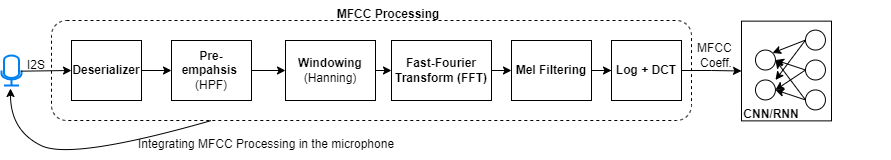
\includegraphics[width=1.0\textwidth]{figs/KWS-arch.png}
    \caption{Keyword Spotter (KWS) architecture.}
    \label{fig:KWS_Arch}
\end{figure}


\section{Example of its Application}
% application (Describe an example consisting of potential application/Future application. This will enable usage model towards its market acceptance) (maximum 200 words)


\section{Benefits and Value Addition}
% (Explain the key benefits of your idea/implementation. You should describe the key value addition of your idea as this will explain why your idea has value in the presence of other participants. It will show uniqueness/Unique selling point/key differentiator) (maximum 200 words)




\section{Team Members}
% •	List your team members’ names, program, department, year of study and contact emails here
\begin{table}[h]
    \centering
    \begin{tabular}{|c|c|c|c|c|}
        \hline
        \textbf{Name} & \textbf{Program} & \textbf{Dept.} & \textbf{Year} & \textbf{Email} \\ \hline\hline
        & & & & \\ \hline
        & & & & \\ \hline
        & & & & \\ \hline
        & & & & \\ \hline
    \end{tabular}
    \caption{Team Member Information}
    \label{tab:student_info}
\end{table}

\section{University Address}
% •	Include the name of your university/college and your institute’s postal address to ship the boards
Silicon University \\
Silicon Hills Road, Patia \\
Bhubaneswar, 751024, ODISHA

\section{Contact Person}
%  Mention one contact person from the institute, his/her official/institute email id, and contact phone number.

Saroj Rout \\
Additional Professor, Electronics Engineering Department \\
Silicon University, Odisha \\
\textit{Email}: \texttt{saroj.rout@silicon.ac.in} \\
\textit{Phone}: +91-90907-52283 \\


\bibliographystyle{ieeetr}
\bibliography{reference}

\end{document}